%%%% CAPÍTULO 2 - REVISÃO DA LITERATURA (OU REVISÃO BIBLIOGRÁFICA, ESTADO DA ARTE, ESTADO DO CONHECIMENTO)
%%
%% O autor deve registrar seu conhecimento sobre a literatura básica do assunto, discutindo e comentando a informação já publicada.
%% A revisão deve ser apresentada, preferencialmente, em ordem cronológica e por blocos de assunto, procurando mostrar a evolução do tema.
%% Título e rótulo de capítulo (rótulos não devem conter caracteres especiais, acentuados ou cedilha)
\chapter{Background}\label{cap:referencialTeorico}

In this section, we'll define in greater detail the theory behind some most
relevant techniques used in the development of the prototype.

This section can be skipped for readers with familiarity on the topics discussed.

\section{Neural Networks}

Neural Networks, or Artificial Neural Networks (\sigla{}{ANN}{Artificial Neural Network}),
are networks built out of interconnected decisional Neurons that aim to replicate 
the behavior of the human brain, enabling computational systems to cluster data
and to make predictions \cite{IBMNeuralNetworks}. 

A Neuron is similar to a Digital Logic Gate, which is capable of producing 
different outputs depending on the input signals that are sent to it.
A Neuron has weights, which are the coefficients that are used for calculating
the outputs; and biases, which are the boundaries that represent how prone is an output
to fit into a specific category of output. 

The main difference between a digital logic gate and a Neuron is that, because neurons are
parameterized with weights and biases, we can apply \textit{learning algorithms}
to tune (or train) Networks of Neurons using real world or synthetic data \cite{Nielsen2015}.

\subsection{Neurons}

One of the most popular types of Neurons is the Perceptron, introduced by 
\cite{Rosenblatt1958} and is shown in Figure \ref{fig:perceptron}. 
A perceptron takes one or more binary inputs and produces a single binary output.

\begin{figure}[H]
	\centering
	\caption[The Perceptron Neuron]{The Perceptron Neuron}
    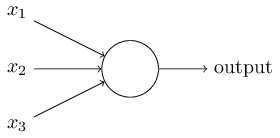
\includegraphics[width=0.5\textwidth]{./images/perceptron.png}
    \fonte{\cite{Nielsen2015}}
	\label{fig:perceptron}
\end{figure}

A Neuron does not necessarily have binary inputs and outputs. In fact,
contemporary systems commonly use a different type of Neuron known as the
Sigmoid Neuron, which take real numbers as inputs and also produces continuous
outputs within the boundaries of the sigmoid curve, shown in Figure
\ref{fig:sigmoid}, instead of discrete zeroes and ones.

This is particularly useful for learning, since in Perceptrons small differences in the 
weights or biases could yield to different outputs without a full transparency 
on how close the output would have been to a different one \cite{Nielsen2015}.

\begin{figure}[H]
	\centering
	\caption[Sigmoid Function]{Sigmoid Function}
    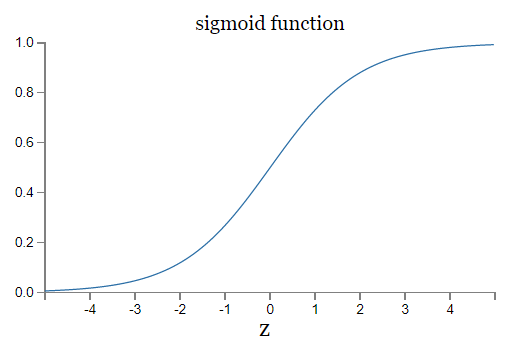
\includegraphics[width=0.5\textwidth]{./images/sigmoid-function.png}
    \fonte{\cite{Nielsen2015}}
	\label{fig:sigmoid}
\end{figure}

\subsection{Learning Algorithms}

There are three main types of learning algorithms: Supervised, Unsupervised and Reinforcement.
Supervised learning is employed when you know what are your expected outputs and use this
information to feed (train) your models such that they can start doing that on their own; 
Unsupervised learning is applied when you do not know what are the expected labels 
in your data or you do not have them available; and Reinforcement learning is used when
algorithms need to replicate specific behaviors depending on the feedback that is
provided to them \cite{CourseraML}. 

Supervised learning is typically employed for regression and classification tasks; 
Unsupervised Learning is typically used for clustering raw data into different buckets
without necessarily knowing how to do it or having the labelled data available;
and Reinforcement learning is often applied in control systems.
This work will primarily focus on Supervised Learning, since our proposed project uses
Object Detection and is trained based on labeled data samples.

As for the learning algorithms used for training Neural Networks, 
the standard algorithm is the Stochastic Gradient Descent (\sigla{SGD}{Stochastic Gradient Descent}).
Alike other gradient descent algorithms, the SGD aims to minimize the loss function of a given
Neural Network iteratively. In simple terms, it consists of an iterative optimization algorithm defined by an
objective function to minimize the error.

The key feature of the SGD is that it does that very efficiently by initializing the weights
and biases randomly and then fine tuning it during training by trying to find the higher descents 
(or the higher derivatives of the error function), reducing the number of necessary iterations, 
which is particularly important considering that the amount of data that is used to train AI
models has increased considerably over the last few years \cite{CornellSGD}.

Finally, in terms of the way how the SGD is computed in Neural Networks, a widely adopted approach 
for Supervised Learning is Backpropagation. Backpropagation computes the gradients of the final 
layers of a Neural Network first, and the gradients of the first layers at last, 
and it reuses partial computations of the gradient from a layer to the other to compute each layer's 
gradient, making it more efficient than calculating each layer's gradient separately \cite{BrilliantBackpropagation}. 

\section{Deep Learning}

Deep Learning defines a group of AI algorithms that use advanced learning techniques on the 
top of ANNs to train models that allow systems to forecast and clusterize data 
efficiently \cite{IBMDeepLearning}.
Deep Learning algorithms use Neural Networks that have three types of layers:
Input Layer, Hidden Layer and Output Layer, shown in Figure \ref{fig:threeLayeredAnn}.
        
\begin{figure}[H]
	\centering
	\caption[Three Layered Neural Network]{Three Layered Neural Network}
    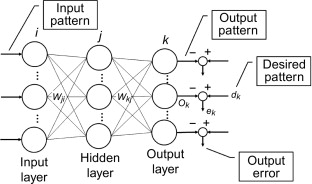
\includegraphics[width=0.6\textwidth]{./images/three-layered-ann.jpg}
    \fonte{\cite{ARAKI2015121}}
	\label{fig:threeLayeredAnn}
\end{figure}

The Input Layer takes the input data that will be fed into the model for training,
$x_i$, and produces the weighting coefficients $w_{ji}$. Input Layers
typically have the role of encoding the input data into a structure that can be processed by the 
subsequent hidden layers \cite{Paranjape2020}.

The $w_{ji}$ coefficients are then used to feed the Hidden Layer of the network,
which produces the weighting coefficients $w_{kj}$. The Hidden Layers of a Deep Learning 
Neural Network are used for the heavy processing of the encoded input data by applying a series of 
mathematical operations that ultimately makes it possible to break down the most important features
of the data and to produce comprehensive outputs to the decisional layers of the network
\cite{DeepAI_HiddenLayer}.

\subsection{Transfer Learning}

Another key technique applied by developers when training Deep Learning models is
\textit{Transfer Learning}. 
It consists of reusing pre-trained networks, which were tuned in other datasets -- usually big and
somehow related to the one that you are going to run your inferences on -- for training custom models.

Transfer Learning works by freezing the weights and biases present in specific layers of a
pre-trained Network -- usually being the hidden layers, which are the feature extractors -- 
when training customized models. This way,  only some layers of the Network -- usually the last layers, which 
are the deciders -- effectively have to be tuned.

The biggest advantages of Transfer Learning are that, because it allows for
training only specific layers of an architecture to get a custom model, the
training process is much faster than it would be if the whole network had to be
retrained; and additionally less training data is required for achieving a good
performing model, since you reuse the work done on the previous training
\cite{CS231N}.

\section{Object Detection}

Images can be processed as number matrices by computers, where each number represents a 
pixel's color level and each index points to a position in the image;
therefore, we can use collections of images as an input to train Deep Learning algorithms 
and perform classification and object detection tasks on them. 

Image Classification is a field of studies that is focused on labeling images
as a whole; Object Detection, on the other hand, focuses not only in
classifying them, but also in identifying the individual label's coordinates
within each image. For the purpose of our project and considering our proposed
product's specifications, we will focus on Object Detection, as it needs to be
able to recognize multiple objects within an image. 

To feed supervised Deep Learning algorithms to detect multiple objects in an
image, we need to provide our AI Models with images that have one or more
labels, the specification on what labels are there, and their coordinates. To
specify the coordinates of an object within an image, we use Bounding Boxes,
shown in Figure \ref{fig:boundingBoxes}. The Bounding Box also describes the
width and height of the object.

\begin{figure}[H]
	\centering
	\caption[Bounding Boxes]{Bounding Boxes}
    \includegraphics[width=0.4\textwidth]{./images/bounding-box.png}
    \fonte{\cite{AmazonRekognition}}
	\label{fig:boundingBoxes}
\end{figure}

For our models to perform feature extraction and ultimately be able to classify
each label in an image and tell their positions, an important mathematical
operation comes to play: the Convolution. Deep Learning algorithms that use
Convolutions in their backbones are typically called Convolutional Neural
Networks (\sigla{CNN}{Convolutional Neural Networks}). These algorithms
typically start by creating grid cells, which are delimiters for groups of
pixels, around the raw images for determining regions of interest and breaking
down concise representations of what are the elements within the image.
Convolutions are then applied from the original image against those grids to
filter and reduce the dimensionality of the original image and create feature
maps \cite{ObjectDetectionDeepLearning}. 

These feature maps then typically go through the final convolutional stages to
calculate Kernels that allows for creating activation functions around the grid
cells that contain each of the objects within the pictures \cite{JeremyJordan};
and those activation functions allow us to determine the Bounding Box
coordinates, the confidence score of the inference and the labels of the image
themselves. 

An example of that process is shown in Figure \ref{fig:convolutionActivation}.

\begin{figure}[H]
	\centering
	\caption[Activation Functions in Object Detection]{Activation Functions in Object Detection}
    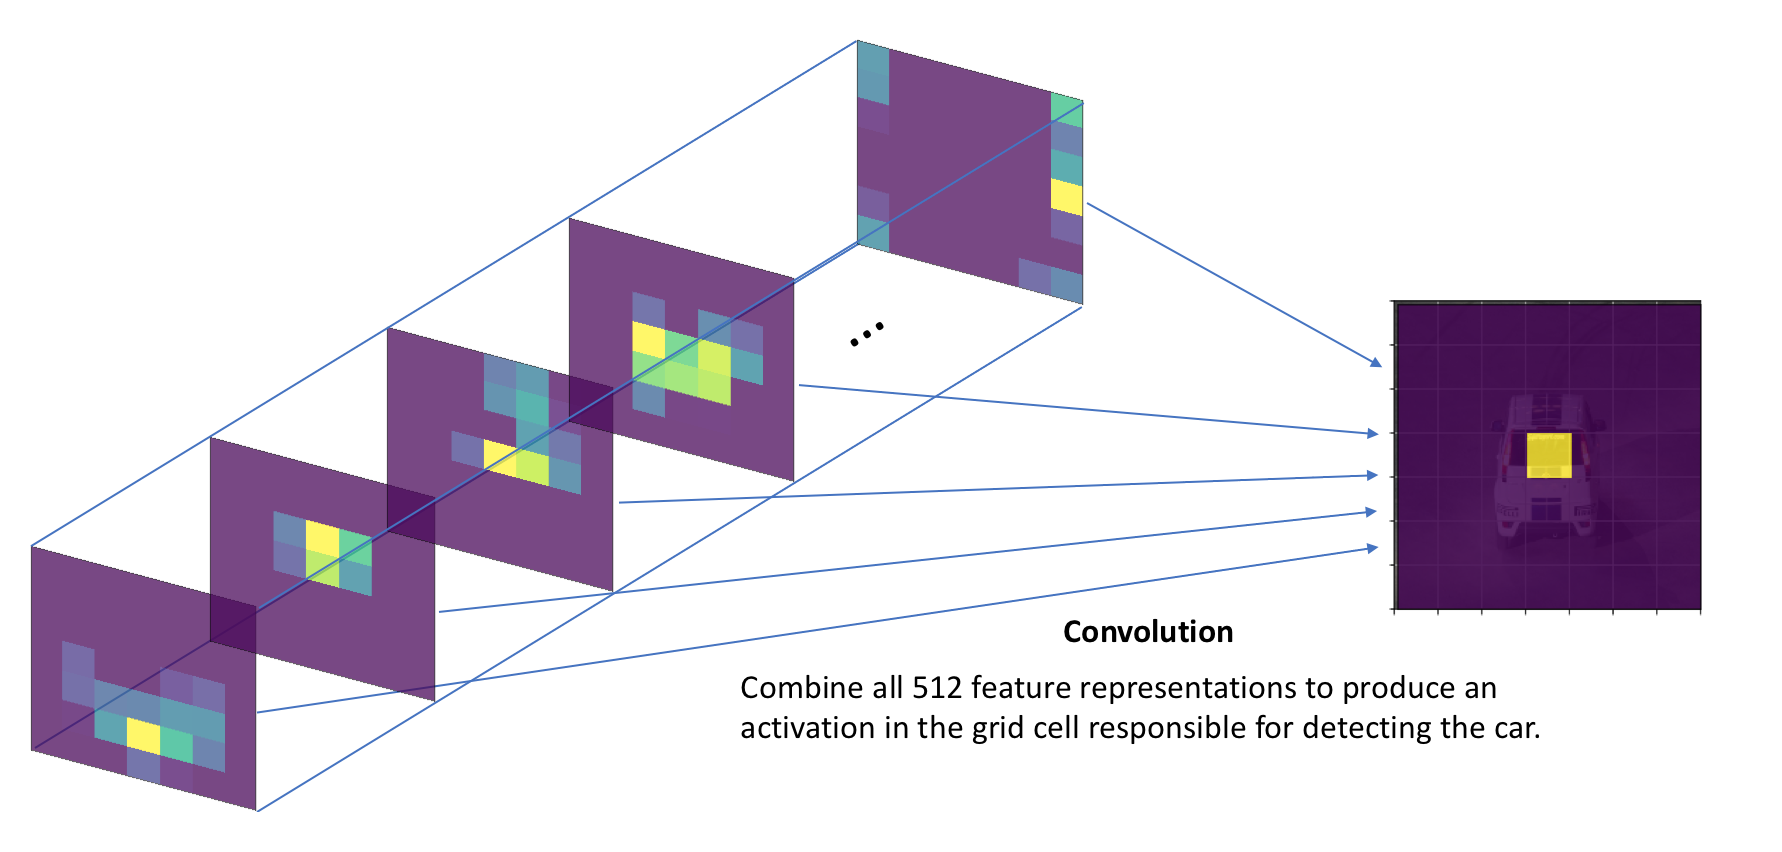
\includegraphics[width=1\textwidth]{./images/convolution-activation.png}
    \fonte{\cite{JeremyJordan}}
	\label{fig:convolutionActivation}
\end{figure}

Finally, a technique known as the Non-Maximum Suppression
(\sigla{NMS}{Non-Maximum Suppression}) is commonly used to filter the regions
of interest with the highest probability scores and ultimately get to a single
bounding box for each prediction. 
An example of the technique is shown in Figure \ref{fig:nmsObjectDetection}.

In this sense, two important metrics used for evaluating Object Detection models
are the Intersection over Union (\sigla{IoU}{Intersection over Union}), which measures 
the overlap between the predicted bounding box and the actual bounding box, 
as shown in Equation \ref{eq:IoU}; and the Average Precision, which measures the percentage 
of correct predictions made by the object detection model, as shown in Equation 
\ref{eq:AP}, where \textbf{True Positives} indicates the number of correct predictions and
\textbf{False Positives} measures the number of incorrect predictions made by the model.

\begin{equation}
\label{eq:IoU}
IoU = \frac{\text{Area of Overlap}}{\text{Area of Union}}=
\frac{
    \tikz{\fill[draw=blue, very thick, fill=blue!20] (0,0) rectangle (1,1) (0.5,-0.5) rectangle (1.5,0.5);
    \fill[draw=blue, very thick, fill=white, even odd rule] (0,0) rectangle (1,1) (0.5,-0.5) rectangle (1.5,0.5);}}
{\tikz{\fill[draw=blue, fill=blue!20, very thick] (0,0) rectangle (1,1) (0.5,-0.5) rectangle (1.5,0.5);}}
\end{equation}

\begin{equation}
	\label{eq:AP}
	AP = \frac{\text{True Positives}}{\text{True Positives + False Positives}}
\end{equation}


\begin{figure}[H]
	\centering
	\caption[NMS Applied to Object Detection]{NMS Applied to Object Detection}
    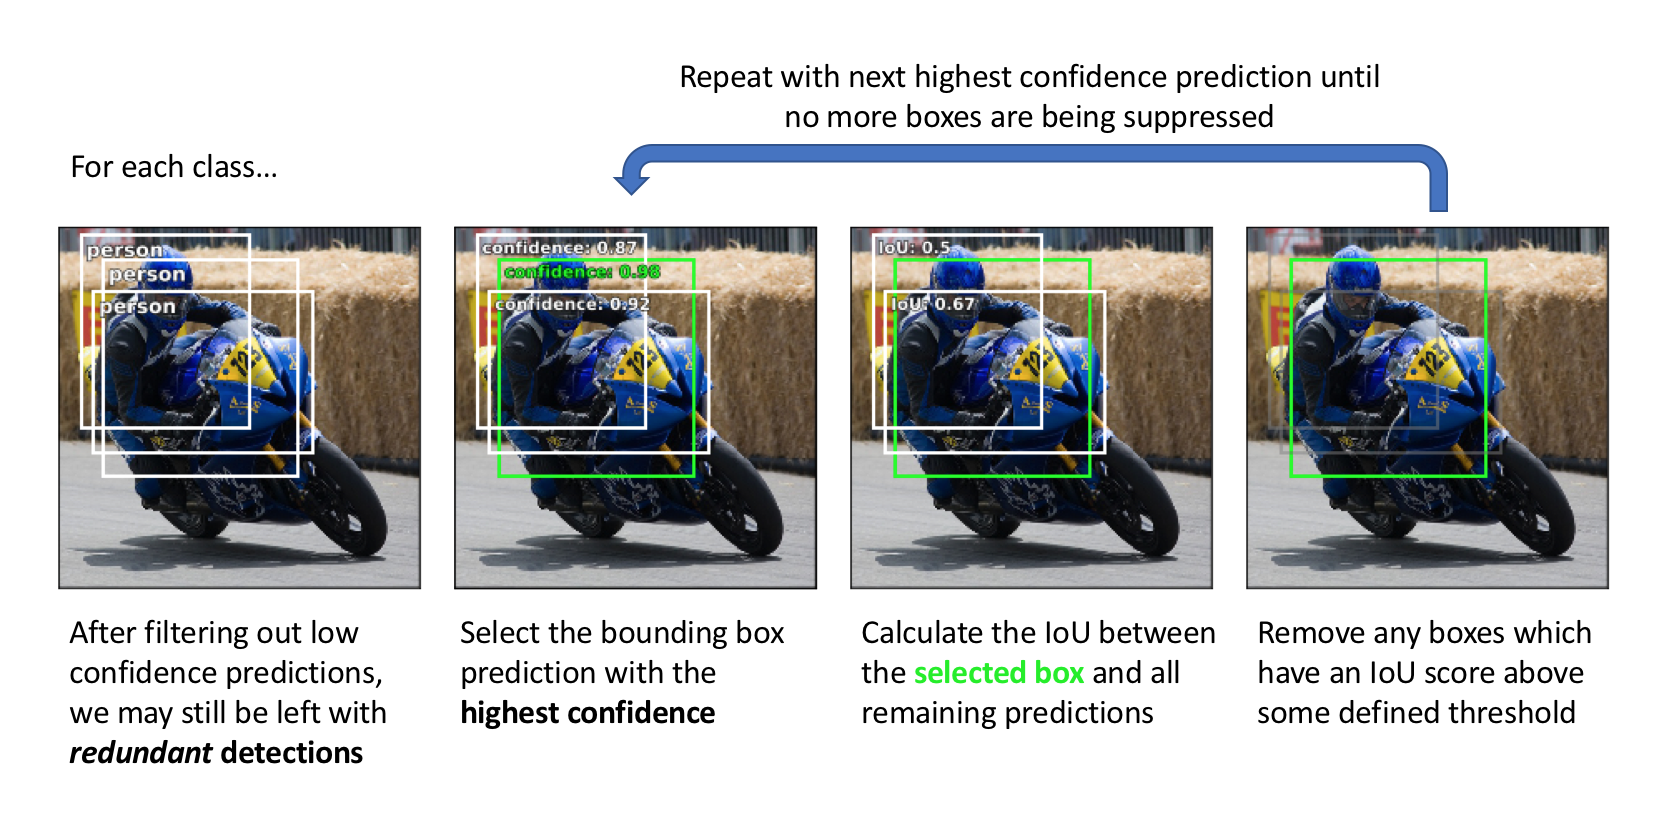
\includegraphics[width=1\textwidth]{./images/nms-object-detection.png }
    \fonte{\cite{JeremyJordan}}
	\label{fig:nmsObjectDetection}
\end{figure}

\section{Tensor Processing Unit}
\label{sec:TPU}

With the increased adoption of Deep Neural Networks (\sigla{DNN}{Deep Neural Networks}) 
in various workloads and their specialized and heavy compute nature, Google started the 
development of a domain specific architecture (\sigla{DSA}{Domain Specific Architecture}) 
which resulted in a first generation custom chip, named Tensor Processing Unit 
(\sigla{TPU}{Tensor Processing Unit}), deployed to their data centers since 2015 \cite{Google2015}.
The developed TPU had the target of improving the inference phase of DNNs and
achieved a performance improvement of \textbf{15-30 times} when compared to
contemporary hardware of paired or reduced power consumption. A block diagram of the TPU
architecture is shown in Figure \ref{fig:tpuarch}.

\begin{figure}[H]
	\centering
	\caption[TPU block diagram]{TPU block diagram. The main computation, matrix multiplication, is done by the yellow units.}
    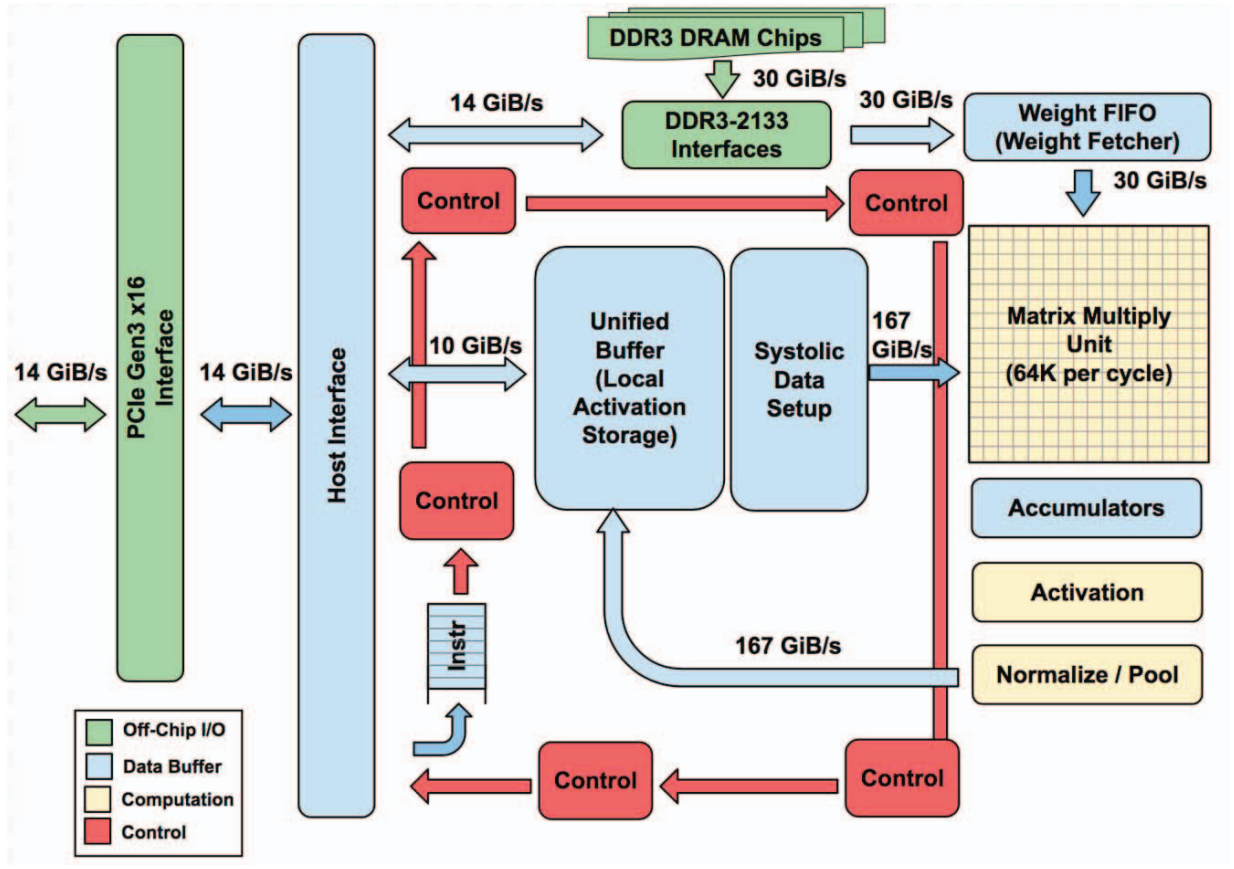
\includegraphics[width=0.6\textwidth]{./images/tpublock.png}
    \fonte{\cite{Google2015}}
	\label{fig:tpuarch}
\end{figure}

Since the first generation TPU described in a 2018 paper \cite{Google2015},
Google has released the TPU into commercials products made available to third
parties. Most notably, the Google Coral\footnote{https://coral.ai} initiative
offers ready-to-use development boards that embedded TPU chips, allowing
developers to leverage the improved DNN performance in their applications.

The Coral Dev Board Micro, an example of those ready-to-use boards is shown in
Figure \ref{fig:coraldev}.

\begin{figure}[H]
	\centering
	\caption[Coral Dev Board Micro]{Coral Dev Board Micro. It includes a microphone, camera and the Coral Edge TPU in a single board package.}
    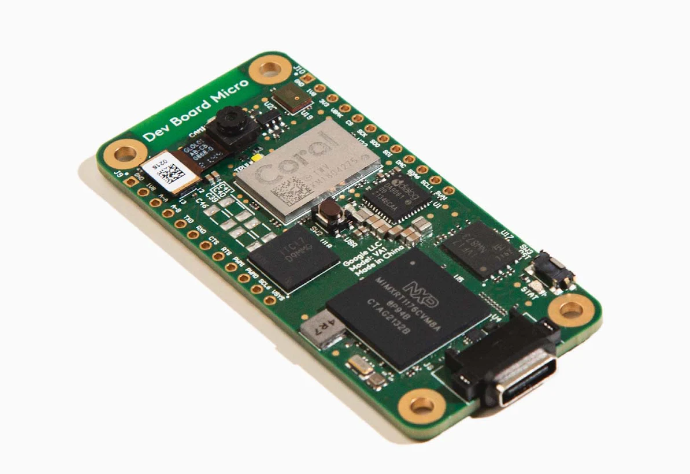
\includegraphics[width=0.5\textwidth]{./images/coralboard.png}
    \fonte{Coral.ai (2022)}
    \label{fig:coraldev}
\end{figure}

\section{Strain Gauge}

For measuring weight, one of the most common transducers used is the strain
gauge. A strain gauge is a device whose measured electrical resistance varies
with changes in its applied force, as a consequence of the mechanical
deformation \cite{Stefanescu}. A typical construction is shown in Figure 
\ref{fig:gauge1}.

\begin{figure}[H]
	\centering
	\caption[Typical Strain Gauge construction]{Typical Strain Gauge construction}
    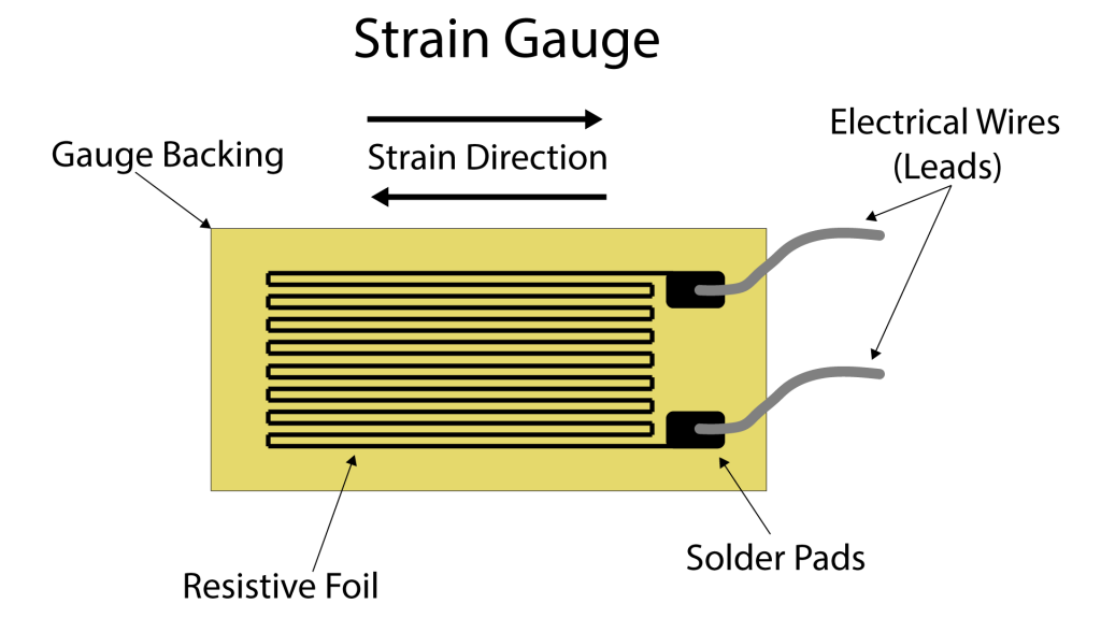
\includegraphics[width=0.5\textwidth]{./images/straingauge.png}
    \fonte{\cite{Michigan2020}}
	\label{fig:gauge1}
\end{figure}

In practice, however, the resistance variations observed after applying a
mechanical strain are minute and can be difficult to measure. To solve that issue,
and to also provide a signal which can be later used as the input of an
Analog-to-Digital Converter (\sigla{ADC}{Analog-to-Digital Converter}), the Wheatstone
Bridge circuit, shown in Figure \ref{fig:gauge2}, can be used \cite{Michigan2020}.

\begin{figure}[H]
	\centering
	\caption[Wheatstone Bridge circuit using four strain gauges]{Wheatstone Bridge circuit using four strain gauges}
    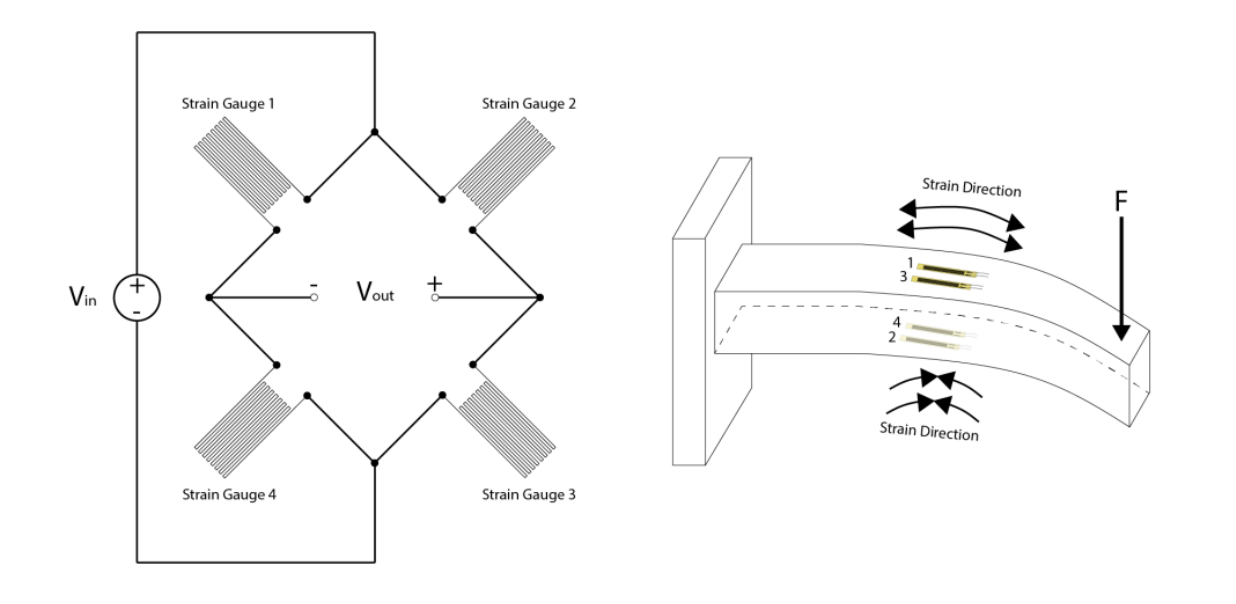
\includegraphics[width=0.9\textwidth]{./images/straingauge2.png}
    \fonte{\cite{Michigan2020}}
	\label{fig:gauge2}
\end{figure}

When no load is applied, the bridge is balanced and the output voltage
$V_{out}$ should be zero. If any strain is applied to the gauges, the bridge
will become unbalanced, and therefore will result in a non-zero output voltage.
Since the voltage variation tends to be small, in the order of millivolts, signal amplification is usually
required for pairing the bridge with commercially available ADCs \cite{HorowitzHill2015}.

It can be shown that the relation between $V_{out}$ and $V_{in}$, $S$, shown on Figure \ref{fig:gauge2}, can be
calculated as \cite{Stefanescu}:

\begin{equation}
    \label{eq:strain}
    S = \frac{V_{out}}{V_{in}} = k\frac{\Delta l}{l}
\end{equation}
where $k$ is known as the \textit{gauge factor}, related to the physical
construction and materials of the strain gauge, and $\frac{\Delta l}{l}$ is the
relative variation of length or strain.

With that, Equation \ref{eq:strain} indicates that the output voltage $V_{out}$
will be linearly proportional to the amount of strain applied, providing the
desired sensing capability.

\section{Load Cell}

Using strain gauges directly can be difficult since a proper
mechanical structure and arrangement is crucial for the sensors to function
properly. For that, commercially available \textit{Load Cells} offer ready to
use mechanical packages that embed the strain gauges for weight sensing
using electronic circuits.

In general, they consist of a spring element onto which the gauges are placed.
When load is applied to the cell, the strain gauges will be stressed and
therefore provide the desired sensing \cite{HBM2022}.

\begin{figure}[H]
	\centering
	\caption[HBM Z6 commercial load cell]{HBM Z6 commercial load cell}
    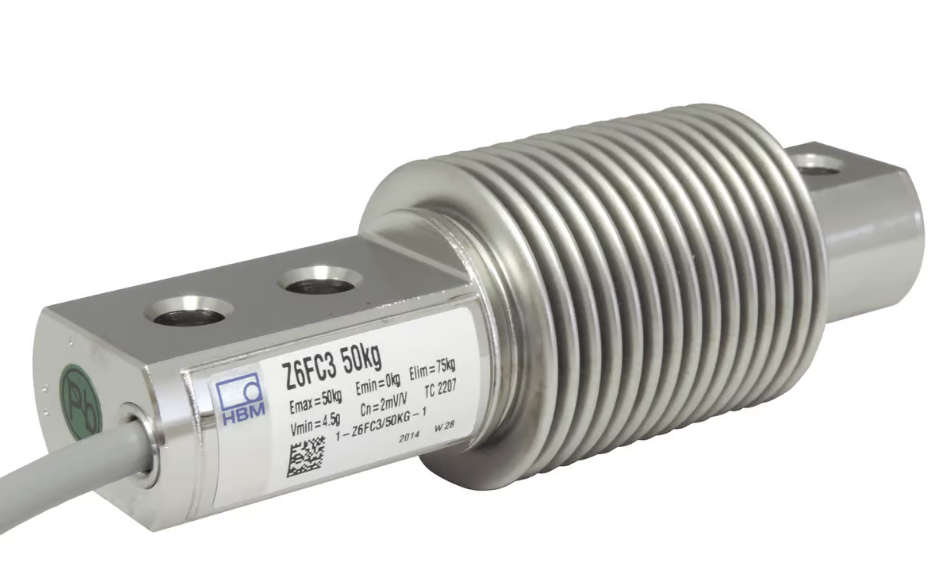
\includegraphics[width=0.3\textwidth]{./images/hbmz6.png}
    \fonte{HBM (2022)}
	\label{fig:gauge2}
\end{figure}
